\documentclass[mathserif]{beamer}

\setbeamertemplate{frametitle}[default][center]%Centers the frame title.
\setbeamertemplate{navigation symbols}{}%Removes navigation symbols.
\setbeamertemplate{footline}{\raisebox{5pt}{\makebox[\paperwidth]{\hfill\makebox[10pt]{\scriptsize\insertframenumber}}}}
\setbeamertemplate{caption}[numbered]

\usepackage{amssymb,amsfonts,amsmath,latexsym,amsthm}
%\usepackage[usenames,dvipsnames]{color}
%\usepackage[]{graphicx}
%\usepackage[space]{grffile}
\usepackage{mathrsfs}   % fancy math font
% \usepackage[font=small,skip=0pt]{caption}
\usepackage[skip=0pt]{caption}
\usepackage{subcaption}
\usepackage{verbatim}
\usepackage{url}
\usepackage{bm}
\usepackage{dsfont}
\usepackage{extarrows}
\usepackage{multirow}
%\newcommand{\tth}   {\mbox{$\theta$}}
\newcommand{\thh}   {\mbox{$\theta$}}
\newcommand{\su}   {\mbox{$\sigma^2$}}
\newcommand{\so}   {\mbox{$\sigma_0^2$}}
\newcommand{\ko}   {\mbox{$\kappa_0$}}
\newcommand{\no}   {\mbox{$\nu_0$}}
\newcommand{\mo}   {\mbox{$\mu_0$}}
\newcommand{\ti}   {\mbox{$\tilde{x}$}}
\newcommand{\la}   {\mbox{$\lambda$}}
\newcommand{\bx}   {\mbox{$\bm{x}$}}
\newcommand{\bZ}   {\mbox{$\bm{Z}$}}
\newcommand{\bX}   {\mbox{$\bm{X}$}}
\newcommand{\bY}   {\mbox{$\bm{Y}$}}
\newcommand{\bA}   {\mbox{$\bm{A}$}}
\newcommand{\ba}   {\mbox{$\bm{a}$}}
\newcommand{\bb}   {\mbox{$\bm{b}$}}
\newcommand{\bt}   {\mbox{$\bm{t}$}}
\newcommand{\bz}   {\mbox{$\bm{z}$}}
\newcommand{\bw}   {\mbox{$\bm{w}$}}
\newcommand{\bbeta}   {\mbox{$\bm{\beta}$}}

\newcommand{\be}   {\mbox{$\bm{e}$}}
\newcommand{\bu}   {\mbox{$\bm{u}$}}
\newcommand{\bv}   {\mbox{$\bm{v}$}}
\newcommand{\sig}   {\mbox{$\Sigma$}}
\newcommand{\sigx}   {\mbox{$\Sigma_{XX}$}}
\newcommand{\sigxy}   {\mbox{$\Sigma_{XY}$}}
\newcommand{\tr}   {\mbox{$\text{tr}$}}
\newcommand{\ddet}   {\mbox{$\text{det}$}}
\newcommand\independent{\protect\mathpalette{\protect\independenT}{\perp}}
\def\independenT#1#2{\mathrel{\rlap{$#1#2$}\mkern2mu{#1#2}}}

\newcommand{\Expect}[1]{\ensuremath{\mathbf{E}\left[ #1 \right]}}
%\newcommand{\Var}[1]{\ensuremath{\mathrm{Var}\left[ #1 \right]}}
%\newcommand{\Cov}[1]{\ensuremath{\mathrm{Cov}\left[ #1 \right]}}
\newcommand{\MSE}{\ensuremath{\mathrm{MSE}}}
\newcommand{\RSS}{\ensuremath{\mathrm{RSS}}}
\newcommand{\Prob}[1]{\ensuremath{\mathrm{Pr}\left( #1 \right)}}
\newcommand{\ProbEst}[1]{\ensuremath{\widehat{\mathrm{Pr}}\left( #1 \right)}}
\DeclareMathOperator*{\argmin}{argmin} % thanks, wikipedia!
\DeclareMathOperator*{\argmax}{argmax} % thanks, wikipedia!
\DeclareMathOperator*{\sgn}{sgn} % thanks, wikipedia!

\newcommand{\lam}{\lambda}
\newcommand{\bmu}{\bm{\mu}}
%\newcommand{\bx}{\ensuremath{\mathbf{X}}}
\newcommand{\X}{\ensuremath{\mathbf{X}}}
\newcommand{\w}{\ensuremath{\mathbf{w}}}
\newcommand{\h}{\ensuremath{\mathbf{h}}}
\newcommand{\V}{\ensuremath{\mathbf{V}}}
%\newcommand{\tr}{\operatorname{tr}}

%\newcommand{\bx}{\ensuremath{\mathbf{X}}}
%\newcommand{\X}{\ensuremath{\mathbf{x}}}
%\newcommand{\w}{\ensuremath{\mathbf{w}}}
%\newcommand{\h}{\ensuremath{\mathbf{h}}}
%\newcommand{\V}{\ensuremath{\mathbf{v}}}
%\newcommand{\Cov}{\text{Cov}}
%\newcommand{\Var}{\text{Var}}

\DeclareMathOperator{\var}{Var}
\DeclareMathOperator{\cov}{Cov}
\newcommand{\Var}[1]{\ensuremath{\mathrm{Var}\left[ #1 \right]}}
\newcommand{\Cov}[1]{\ensuremath{\mathrm{Cov}\left[ #1 \right]}}


\newcommand{\indep}{\rotatebox{90}{\ensuremath{\models}}}
\newcommand{\notindep}{\not\hspace{-.05in}\indep}







\usepackage{float,bm}
\floatstyle{boxed}
\newfloat{code}{tp}{code}
\floatname{code}{Code Example}
%\newcommand{\tth}   {\mbox{$\theta$}}
\newcommand{\thh}   {\mbox{$\theta$}}
\newcommand{\su}   {\mbox{$\sigma^2$}}
\newcommand{\so}   {\mbox{$\sigma_0^2$}}
\newcommand{\ko}   {\mbox{$\kappa_0$}}
\newcommand{\no}   {\mbox{$\nu_0$}}
\newcommand{\mo}   {\mbox{$\mu_0$}}
\newcommand{\ti}   {\mbox{$\tilde{x}$}}
\newcommand{\la}   {\mbox{$\lambda$}}
\newcommand{\bx}   {\mbox{$\bm{x}$}}
\newcommand{\bZ}   {\mbox{$\bm{Z}$}}
\newcommand{\bX}   {\mbox{$\bm{X}$}}
\newcommand{\bY}   {\mbox{$\bm{Y}$}}
\newcommand{\bA}   {\mbox{$\bm{A}$}}
\newcommand{\ba}   {\mbox{$\bm{a}$}}
\newcommand{\bb}   {\mbox{$\bm{b}$}}
\newcommand{\bt}   {\mbox{$\bm{t}$}}
\newcommand{\bz}   {\mbox{$\bm{z}$}}
\newcommand{\bw}   {\mbox{$\bm{w}$}}
\newcommand{\bbeta}   {\mbox{$\bm{\beta}$}}

\newcommand{\be}   {\mbox{$\bm{e}$}}
\newcommand{\bu}   {\mbox{$\bm{u}$}}
\newcommand{\bv}   {\mbox{$\bm{v}$}}
\newcommand{\sig}   {\mbox{$\Sigma$}}
\newcommand{\sigx}   {\mbox{$\Sigma_{XX}$}}
\newcommand{\sigxy}   {\mbox{$\Sigma_{XY}$}}
\newcommand{\tr}   {\mbox{$\text{tr}$}}
\newcommand{\ddet}   {\mbox{$\text{det}$}}
\newcommand\independent{\protect\mathpalette{\protect\independenT}{\perp}}
\def\independenT#1#2{\mathrel{\rlap{$#1#2$}\mkern2mu{#1#2}}}

\newcommand{\Expect}[1]{\ensuremath{\mathbf{E}\left[ #1 \right]}}
%\newcommand{\Var}[1]{\ensuremath{\mathrm{Var}\left[ #1 \right]}}
%\newcommand{\Cov}[1]{\ensuremath{\mathrm{Cov}\left[ #1 \right]}}
\newcommand{\MSE}{\ensuremath{\mathrm{MSE}}}
\newcommand{\RSS}{\ensuremath{\mathrm{RSS}}}
\newcommand{\Prob}[1]{\ensuremath{\mathrm{Pr}\left( #1 \right)}}
\newcommand{\ProbEst}[1]{\ensuremath{\widehat{\mathrm{Pr}}\left( #1 \right)}}
\DeclareMathOperator*{\argmin}{argmin} % thanks, wikipedia!
\DeclareMathOperator*{\argmax}{argmax} % thanks, wikipedia!
\DeclareMathOperator*{\sgn}{sgn} % thanks, wikipedia!

\newcommand{\lam}{\lambda}
\newcommand{\bmu}{\bm{\mu}}
%\newcommand{\bx}{\ensuremath{\mathbf{X}}}
\newcommand{\X}{\ensuremath{\mathbf{X}}}
\newcommand{\w}{\ensuremath{\mathbf{w}}}
\newcommand{\h}{\ensuremath{\mathbf{h}}}
\newcommand{\V}{\ensuremath{\mathbf{V}}}
%\newcommand{\tr}{\operatorname{tr}}

%\newcommand{\bx}{\ensuremath{\mathbf{X}}}
%\newcommand{\X}{\ensuremath{\mathbf{x}}}
%\newcommand{\w}{\ensuremath{\mathbf{w}}}
%\newcommand{\h}{\ensuremath{\mathbf{h}}}
%\newcommand{\V}{\ensuremath{\mathbf{v}}}
%\newcommand{\Cov}{\text{Cov}}
%\newcommand{\Var}{\text{Var}}

\DeclareMathOperator{\var}{Var}
\DeclareMathOperator{\cov}{Cov}
\newcommand{\Var}[1]{\ensuremath{\mathrm{Var}\left[ #1 \right]}}
\newcommand{\Cov}[1]{\ensuremath{\mathrm{Cov}\left[ #1 \right]}}


\newcommand{\indep}{\rotatebox{90}{\ensuremath{\models}}}
\newcommand{\notindep}{\not\hspace{-.05in}\indep}






%\usepackage{fontspec}
%\setmainfont{Tahoma}

%\newcommand{\lam}{\lambda}
%\newcommand{\bmu}{\bm{\mu}}
%%\newcommand{\bx}{\ensuremath{\mathbf{X}}}
%\newcommand{\X}{\ensuremath{\mathbf{x}}}
%\newcommand{\w}{\ensuremath{\mathbf{w}}}
%\newcommand{\h}{\ensuremath{\mathbf{h}}}
%\newcommand{\V}{\ensuremath{\mathbf{v}}}
%\newcommand{\cov}{\text{Cov}}
%\newcommand{\var{\text{Var}}}

%\DeclareMathOperator{\var}{Var}
%\DeclareMathOperator{\cov}{Cov}

%\newcommand{\indep}{\rotatebox{90}{\ensuremath{\models}}}
%\newcommand{\notindep}{\not\hspace{-.05in}\indep}

\usepackage{graphicx} %The mode "LaTeX => PDF" allows the following formats: .jpg  .png  .pdf  .mps
\graphicspath{{./PresentationPictures/}} %Where the figures folder is located
\usepackage{listings}
\usepackage{media9}
\usepackage{movie15}
\addmediapath{./Movies/}

\newcommand{\beginbackup}{
   \newcounter{framenumbervorappendix}
   \setcounter{framenumbervorappendix}{\value{framenumber}}
}
\newcommand{\backupend}{
   \addtocounter{framenumbervorappendix}{-\value{framenumber}}
   \addtocounter{framenumber}{\value{framenumbervorappendix}} 
}


%\usepackage{algorithm2e}
\usepackage[ruled,lined]{algorithm2e}
\def\algorithmautorefname{Algorithm}
\SetKwIF{If}{ElseIf}{Else}{if}{then}{else if}{else}{endif}
%\usepackage{times}
%\usepackage[tbtags]{amsmath}
%\usepackage{amssymb}
\usepackage{amsfonts}
%\usepackage{slfortheorems}
\usepackage{epsfig}
\usepackage{graphicx}
%\usepackage[small]{caption}
%\usepackage[square]{natbib}
%\newcommand{\newblock}{}
%\bibpunct{(}{)}{;}{a}{}{,}
%\bibliographystyle{ims}
%\usepackage[letterpaper]{geometry}
%\usepackage{color}
%\setlength{\parindent}{0pt}

\usepackage{natbib}
\bibpunct{(}{)}{;}{a}{}{,}
%\usepackage{hyperref}

\DeclareMathOperator*{\Exp}{Exp}
\DeclareMathOperator*{\TExp}{TExp}
\DeclareMathOperator*{\Bernoulli}{Bernoulli}
\DeclareMathOperator*{\Beta}{Beta}
\DeclareMathOperator*{\Ga}{Gamma}
\DeclareMathOperator*{\TGamma}{TGamma}
\DeclareMathOperator*{\Poisson}{Poisson}
\DeclareMathOperator*{\Binomial}{Binomial}
\DeclareMathOperator*{\NormalGamma}{NormalGamma}
\DeclareMathOperator*{\InvGamma}{InvGamma}
\DeclareMathOperator*{\Cauchy}{Cauchy}
\DeclareMathOperator*{\Uniform}{Uniform}
\DeclareMathOperator*{\Gumbel}{Gumbel}
\DeclareMathOperator*{\Pareto}{Pareto}
\DeclareMathOperator*{\Mono}{Mono}
\DeclareMathOperator*{\Geometric}{Geometric}
\DeclareMathOperator*{\Wishart}{Wishart}

\newcommand{\R}{\mathbb{R}}
\newcommand{\Z}{\mathbb{Z}}
\newcommand{\E}{\mathbb{E}}
\renewcommand{\Pr}{\mathbb{P}}
\newcommand{\I}{\mathds{1}}
\newcommand{\V}{\mathbb{V}}

% Math operators
\DeclareMathOperator*{\diag}{diag}
\DeclareMathOperator*{\median}{median}
\DeclareMathOperator*{\Vol}{Vol}

% Miscellaneous commands
\newcommand{\iid}{\stackrel{\mathrm{iid}}{\sim}}
\newcommand{\matrixsmall}[1]{\bigl(\begin{smallmatrix}#1\end{smallmatrix} \bigr)}

\newcommand{\items}[1]{\begin{itemize} #1 \end{itemize}}

\newcommand{\todo}[1]{\emph{\textcolor{red}{(#1)}}}

\newcommand{\branch}[4]{
\left\{
	\begin{array}{ll}
		#1  & \mbox{if } #2 \\
		#3 & \mbox{if } #4
	\end{array}
\right.
}

% approximately proportional to
\def\app#1#2{%
  \mathrel{%
    \setbox0=\hbox{$#1\sim$}%
    \setbox2=\hbox{%
      \rlap{\hbox{$#1\propto$}}%
      \lower1.3\ht0\box0%
    }%
    \raise0.25\ht2\box2%
  }%
}
\def\approxprop{\mathpalette\app\relax}

\newcommand{\btheta}{{\bm\theta}}
\newcommand{\bbtheta}{{\pmb{\bm\theta}}}

%\usepackage{zref-savepos}
%
%\newcounter{restofframe}
%\newsavebox{\restofframebox}
%\newlength{\mylowermargin}
%\setlength{\mylowermargin}{2pt}
%
%\newenvironment{restofframe}{%
%    \par%\centering
%    \stepcounter{restofframe}%
%    \zsavepos{restofframe-\arabic{restofframe}-begin}%
%    \begin{lrbox}{\restofframebox}%
%}{%
%    \end{lrbox}%
%    \setkeys{Gin}{keepaspectratio}%
%    \raisebox{\dimexpr-\height+\ht\strutbox\relax}[0pt][0pt]{%
%    \resizebox*{!}{\dimexpr\zposy{restofframe-\arabic{restofframe}-begin}sp-\zposy{restofframe-\arabic{restofframe}-end}sp-\mylowermargin\relax}%
%        {\usebox{\restofframebox}}%
%    }%
%    \vskip0pt plus 1filll\relax
%    \mbox{\zsavepos{restofframe-\arabic{restofframe}-end}}%
%    \par
%}


\usepackage{tikz}
\usetikzlibrary{arrows}

%\usepackage[usenames,dvipsnames]{xcolor}
\usepackage{tkz-berge}
\usetikzlibrary{fit,shapes}

\usepackage{calc}
%%
%% The tikz package is used for doing the actual drawing.
%\usepackage{tikz}
%%
%% In order to be able to put arrowheads in the middle of directed edges, we need an extra library.
\usetikzlibrary{decorations.markings}
%%
%% The next line says how the "vertex" style of nodes should look: drawn as small circles.
\tikzstyle{vertex}=[circle, draw, inner sep=0pt, minimum size=6pt]
%%
%% Next, we make a \vertex command as a shorthand in place of \node[vertex} to get that style.
\newcommand{\vertex}{\node[vertex]}
%%
%% Finally, we declare a "counter", which is what LaTeX calls an integer variable, for use in
%% the calculations of angles for evenly spacing vertices in circular arrangements.
\newcounter{Angle}

\newtheoremstyle{example}
{\topsep} % space above
{\topsep} % space below
{} % body font
{} % indent
{\bf} % head font
{:} % punctuation between head and body
{0.5em} % space after head
{} % manually specify head
%{\thmname{#1}\thmnumber{ #2}\thmnote{:#3}} % manually specify head

\theoremstyle{example}
\newtheorem{ex}{Example}[section]

\newtheoremstyle{definition}
{\topsep} % space above
{\topsep} % space below
{} % body font
{} % indent
{\sc} % head font
{:} % punctuation between head and body
{0.5em} % space after head
{} % manually specify head
%{\thmname{#1}\thmnumber{ #2}\thmnote{:#3}} % manually specify head

\theoremstyle{definition}
\newtheorem{defn}{Definition}[section]

\theoremstyle{rem}
\newtheorem{rem}{Remark}[section]

\newtheoremstyle{theorem}
{\topsep} % space above
{\topsep} % space below
{} % body font
{} % indent
{\sc} % head font
{:} % punctuation between head and body
{0.5em} % space after head
{} % manually specify head
%{\thmname{#1}\thmnumber{ #2}\thmnote{:#3}} % manually specify head

\theoremstyle{theorm}
\newtheorem{thm}{Theorem}[section]



%%%to add in new counter for slides in beamer

%\setbeamertemplate{footline}{
%  \leavevmode%
%  \hbox{%
%  \begin{beamercolorbox}[wd=.333333\paperwidth,ht=2.25ex,dp=1ex,center]{author in head/foot}%
%    \usebeamerfont{author in head/foot}\insertshortauthor~~(\insertshortinstitute)
%  \end{beamercolorbox}%
%  \begin{beamercolorbox}[wd=.333333\paperwidth,ht=2.25ex,dp=1ex,center]{title in head/foot}%
%    \usebeamerfont{title in head/foot}\insertshorttitle
%  \end{beamercolorbox}%
%  \begin{beamercolorbox}[wd=.333333\paperwidth,ht=2.25ex,dp=1ex,right]{date in head/foot}%
%    \usebeamerfont{date in head/foot}\insertshortdate{}\hspace*{2em}
%    \insertframenumber{} \hspace*{2ex} % hier hat's sich ge�ndert
%  \end{beamercolorbox}}%
%  \vskip0pt%
%}



%%%%%

\newcommand*\oldmacro{}
\let\oldmacro\insertshortauthor
\renewcommand*\insertshortauthor{
  \leftskip=.3cm
\insertframenumber\,/\,\inserttotalframenumber\hfill\oldmacro}




%\excludecomment{notbeamer}
%\includecomment{beamer}



\title{Intro to Monte Carlo, Part II}
\author{Rebecca C. Steorts \\ Bayesian Methods and Modern Statistics: STA 360/601}
\date{Module 5}



\begin{document}
\maketitle

\frame{
\frametitle{Rejection Sampling}

Rejection sampling is a method for drawing random samples from a distribution whose p.d.f.\ can be evaluated up to a constant of proportionality. 

%\vskip 1 em
%Compared with the inverse c.d.f.\ method, rejection sampling has the advantage of working on complicated multivariate distributions.

\vskip 1 em

Difficulties? You must design a good proposal distribution (which can be difficult, especially in high-dimensional settings).

}

\frame{
\frametitle{Uniform Sampler}

Goal: Generate samples from Uniform(A), where A is complicated. 

\vskip 1 em

Example: $X \sim $ Uniform(Mandelbrot).

\vskip 1 em

How? Consider $I_X(A).$


\begin{figure}
  \begin{center}
    
\includegraphics[width=0.45\textwidth]{madel}
%    \hspace{0.05\textwidth}
%    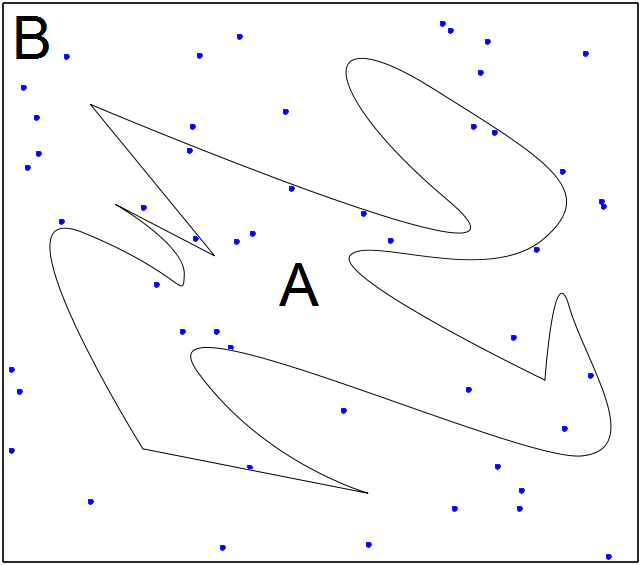
\includegraphics[width=0.45\textwidth]{code/reject-w-samples.png}
%    % Source: Original work by Jeffrey W. Miller
%    % Date: 2/1/2014
  \end{center}
  \caption{A complicated function $A,$ called the Mandelbrot!}
%  \label{figure:reject}
\end{figure}


}

\frame{
\frametitle{Proposition}
\begin{itemize}
\item Suppose $A \subset B.$ 
\item Let $Y_1,Y_2,\ldots \sim$ Uniform(B) iid and
\item  $X = Y_k$
where $k= \min \{k: Y_k \in A\},$ 
\end{itemize}
Then it follows that
$$X \sim \text{Uniform}(A).$$

Proof: Exercise. Hint: Try the discrete case first and use a geometric series. 



}

\frame{

\begin{figure}
  \begin{center}
    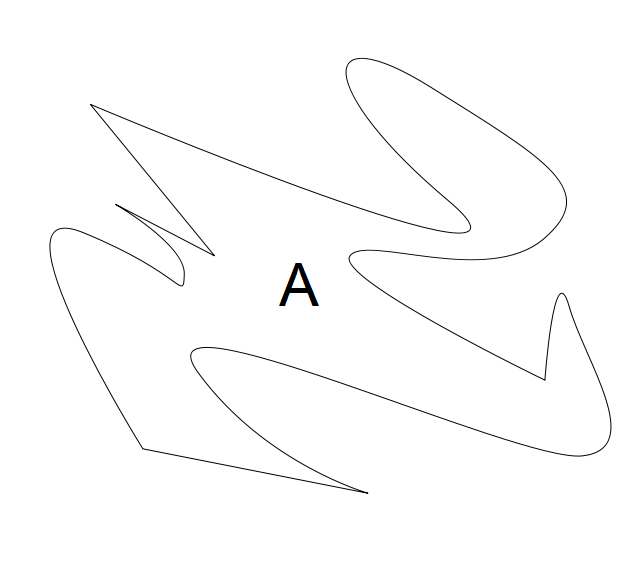
\includegraphics[width=0.45\textwidth]{code/reject-wo-samples.png}
    \hspace{0.05\textwidth}
    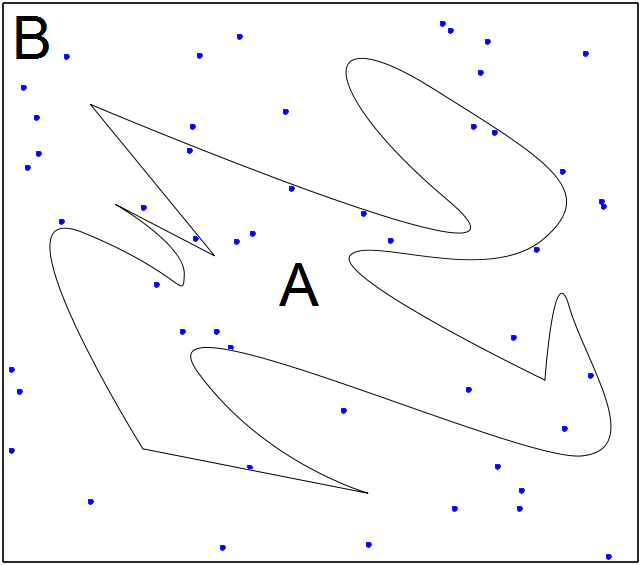
\includegraphics[width=0.45\textwidth]{code/reject-w-samples.png}
    % Source: Original work by Jeffrey W. Miller
    % Date: 2/1/2014
  \end{center}
  \caption{(Left) How to draw uniform samples from region $A$? (Right) Draw uniform samples from $B$ and keep only those that are in $A$.}
  \label{figure:reject}
\end{figure}

}

%\frame{
%\frametitle{Simple Rejection Sampling Formally Written}
%\begin{itemize}
%\item Let $\pi$ be a density. Suppose $$\pi(x) = c \;\ell(x),$$ where $\ell$ is known, $c$ is  unknown. 
%\item We are interested in case where \textcolor{blue}{$\pi$ is complicated}.
%\item Goal: Generate $X \sim \pi.$
%\end{itemize}
%
%{Simple rejection sampling}
%\begin{itemize}
%\item We're going to place a ``uniform box" over $\pi(x)$.
%\item Assume $\ell(x)$ is bounded and is zero outside of $[0, 1].$
%\item Suppose also $\ell(x)$ is constant on the intervals $$((j - 1)/k, j/k), j = 1,\ldots, k.$$ 
%\item Let $M$ be such that $M \geq \ell(x)$ for all $x.$
%\end{itemize}
%
%
%}

%\frame{
%\frametitle{Simple Rejection Sampling Algorithm}
%For very the very simple case, consider the following procedure.
%\begin{enumerate}
%\item Generate a point $(U_1, U_2)$ uniformly at random from the rectangle of
%height $M$ sitting on top of the interval $[0, 1].$
%\item If the point is below the graph of the function $\ell$, retain $U_1.$ Else, reject the point and go back to (1).
%\end{enumerate}
%
%\vskip 1 em
%
%Remark: Using the Probability Integral Transformation in reverse. If $X \sim F^{-1}(U),$ then $X \sim F$ where $U \sim \text{Uniform}(0,1).$
%
%\vskip 1 em
%
%%Remark: Think about what this is doing, we're generating many draws that are wasting time. Think about the restriction on $[0,1]$ and if this makes sense. 
%
%}

\frame{
\frametitle{General Rejection Sampling Algorithm}
%Let $\pi$ be a density. Suppose $$\pi(x) = c \;\ell(x),$$ where $\ell$ is known, $c$ is  unknown. 
Goal: Sample from a \textcolor{red}{complicated pdf $f(x).$}
\vskip 1 em
Suppose that $$\textcolor{red}{f(x)} = \tilde{f}(x)/\alpha, \alpha>0$$.

Algorithm: 


%Suppose the density $g$ is such that for some known constant $M,$ 
%$$Mg(x) \geq \ell(x)$$ for all $x.$
%Procedure:
\begin{enumerate}
\item Choose a \textcolor{blue}{proposal distribution $q$} such that $c>0$ with 
$$c \textcolor{blue}{q(x)} \geq \tilde{f}(x).$$
\item Sample $X \sim \textcolor{blue}{q}$, sample $Y \sim \text{Unif}(0, c\; \textcolor{blue}{q(X)})$ (given X)
\item If $Y \leq \tilde{f}(X), Z=X,$\\
Otherwise we reject and return to step (2). 
%Generate $X \sim g,$ and calculate $r(X) = \dfrac{\ell(X)}{M\; g(X)}.$
%\item Flip a coin with probability of success $r(X).$ If we have a success,
%retain X. Else return to (1).
\end{enumerate}
Output: $Z \sim f$\\
Proof: Exercise.
}
%\frame{
%\frametitle{General Rejection Sampling Algorithm}
%To show that an accepted point has distribution $\pi$, let \textcolor{blue}{$I$ be the indicator that
%the point is accepted.} Then
%\begin{align}
%P(I=1) &= \int P(I=1 \mid X=x) g(x) \; dx\\
%& = \int \frac{\ell(x)}{M\; g(x)} g(x)\; dx \\
%&= \int \frac{\pi(x)/c}{M\; g(x)} g(x)\; dx \\
%&= 
%\frac{1}{c\; M} \int \pi(x) \; dx \\
%&= 
%\frac{1}{c\; M}.
%\end{align}
%
%Thus, if $g_\ell$ is the conditional distribution of $X$ given $I,$ we have
%\begin{align}
%g_I(x | I=1) &= P(x, I = 1)/ P(I=1)\\
%&=
%g(x) \frac{\pi(x)/c}{M\; g(x)} / P(I=1) = \pi(x).
%\end{align}
%}

\frame{


\begin{figure}
  \begin{center}
    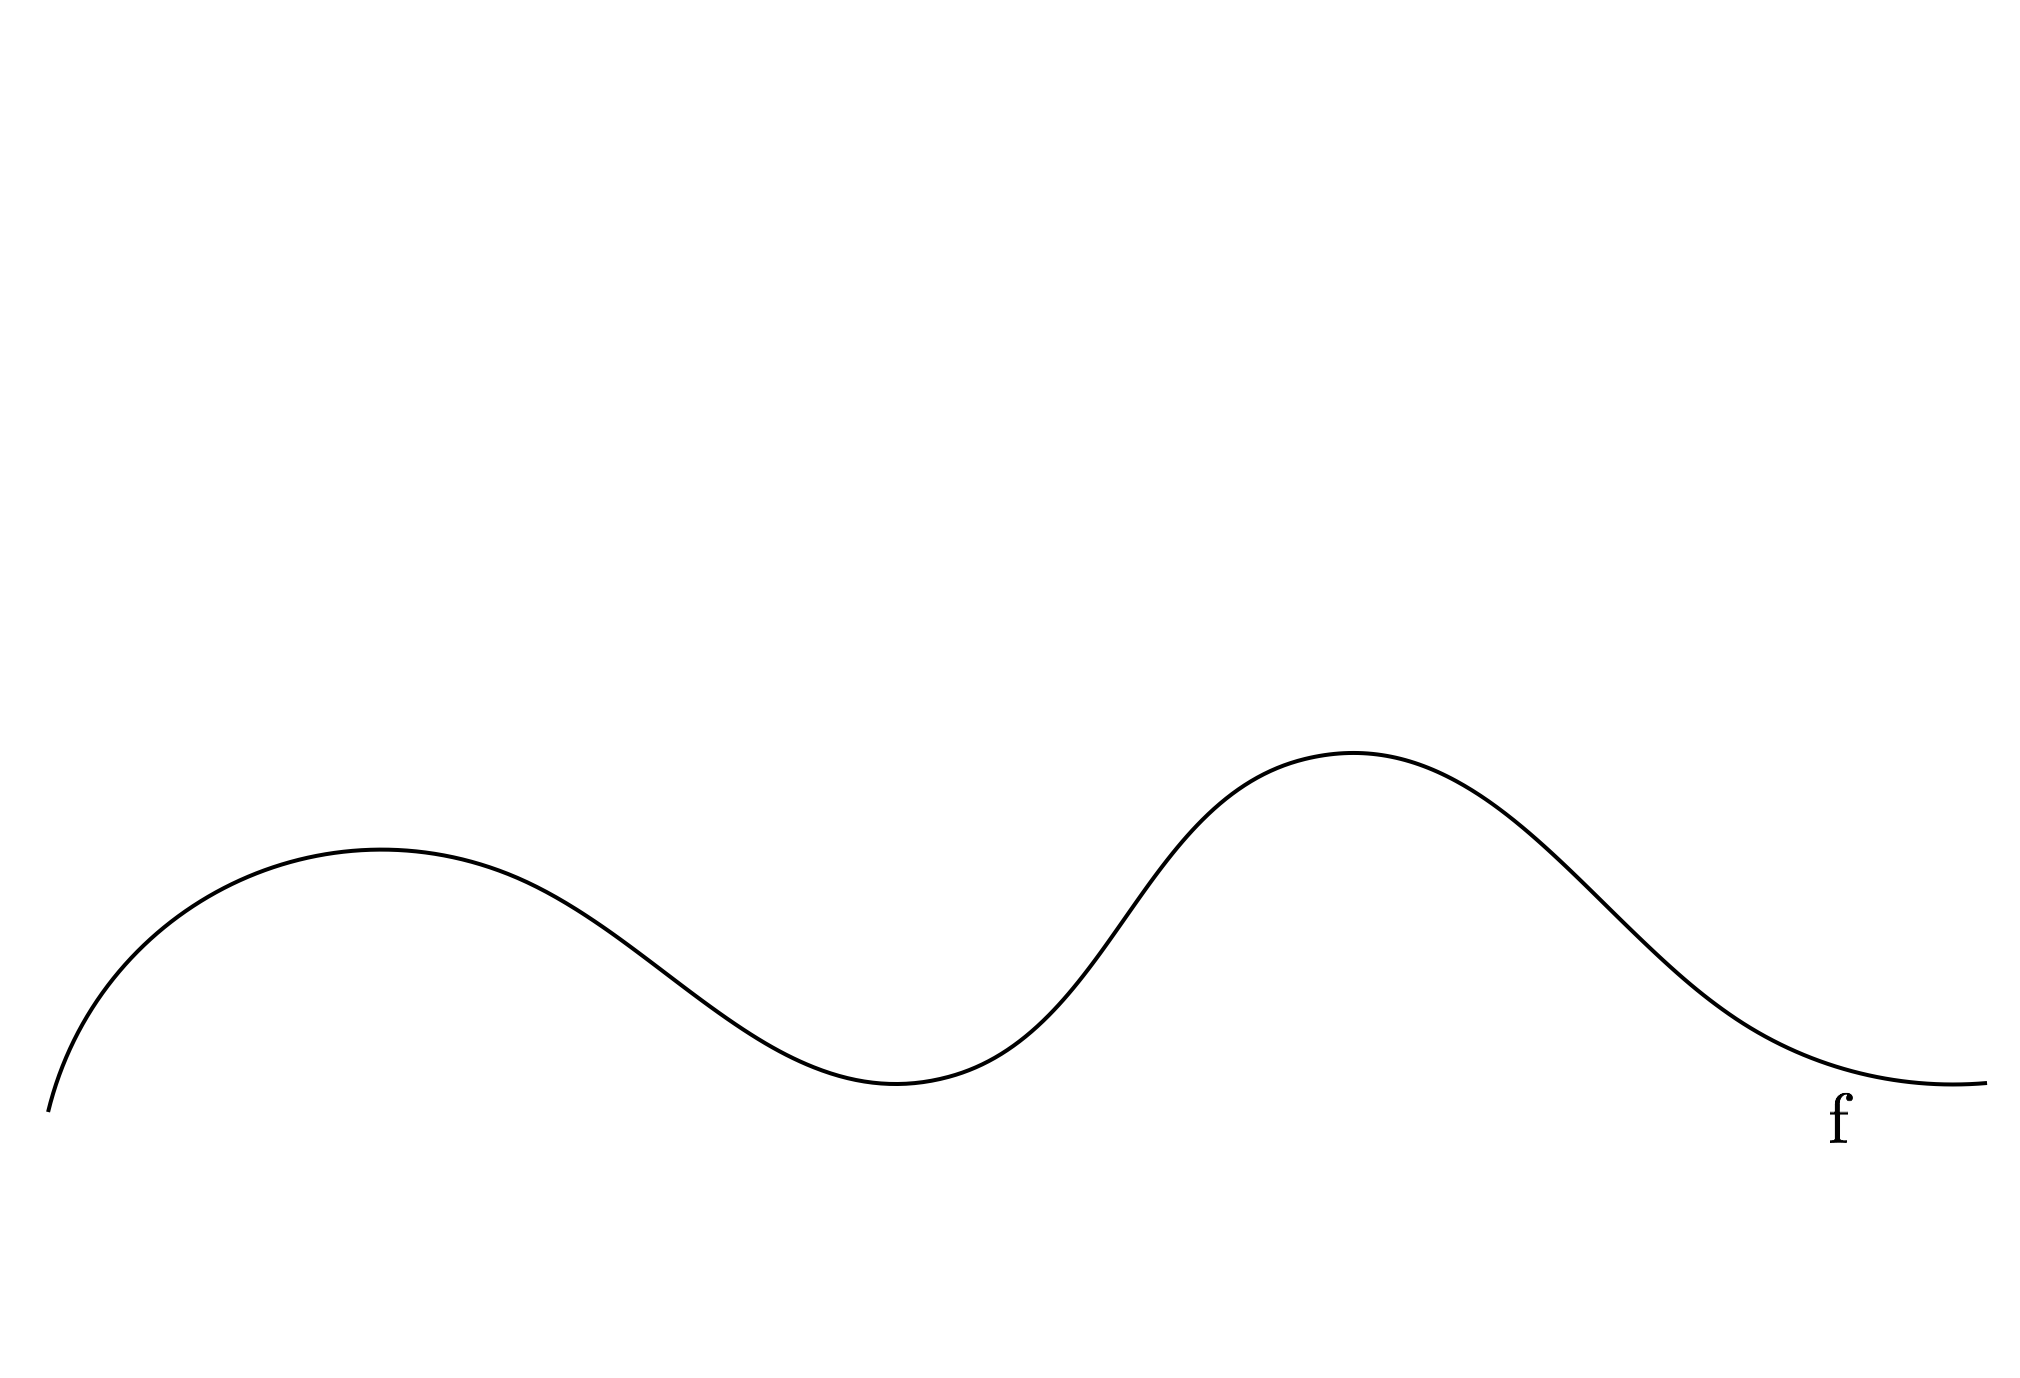
\includegraphics[width=0.8\textwidth]{f}
  \end{center}
  \caption{Visualizing just f (hard to sample from).}
\end{figure}



}

\frame{


\begin{figure}
  \begin{center}
    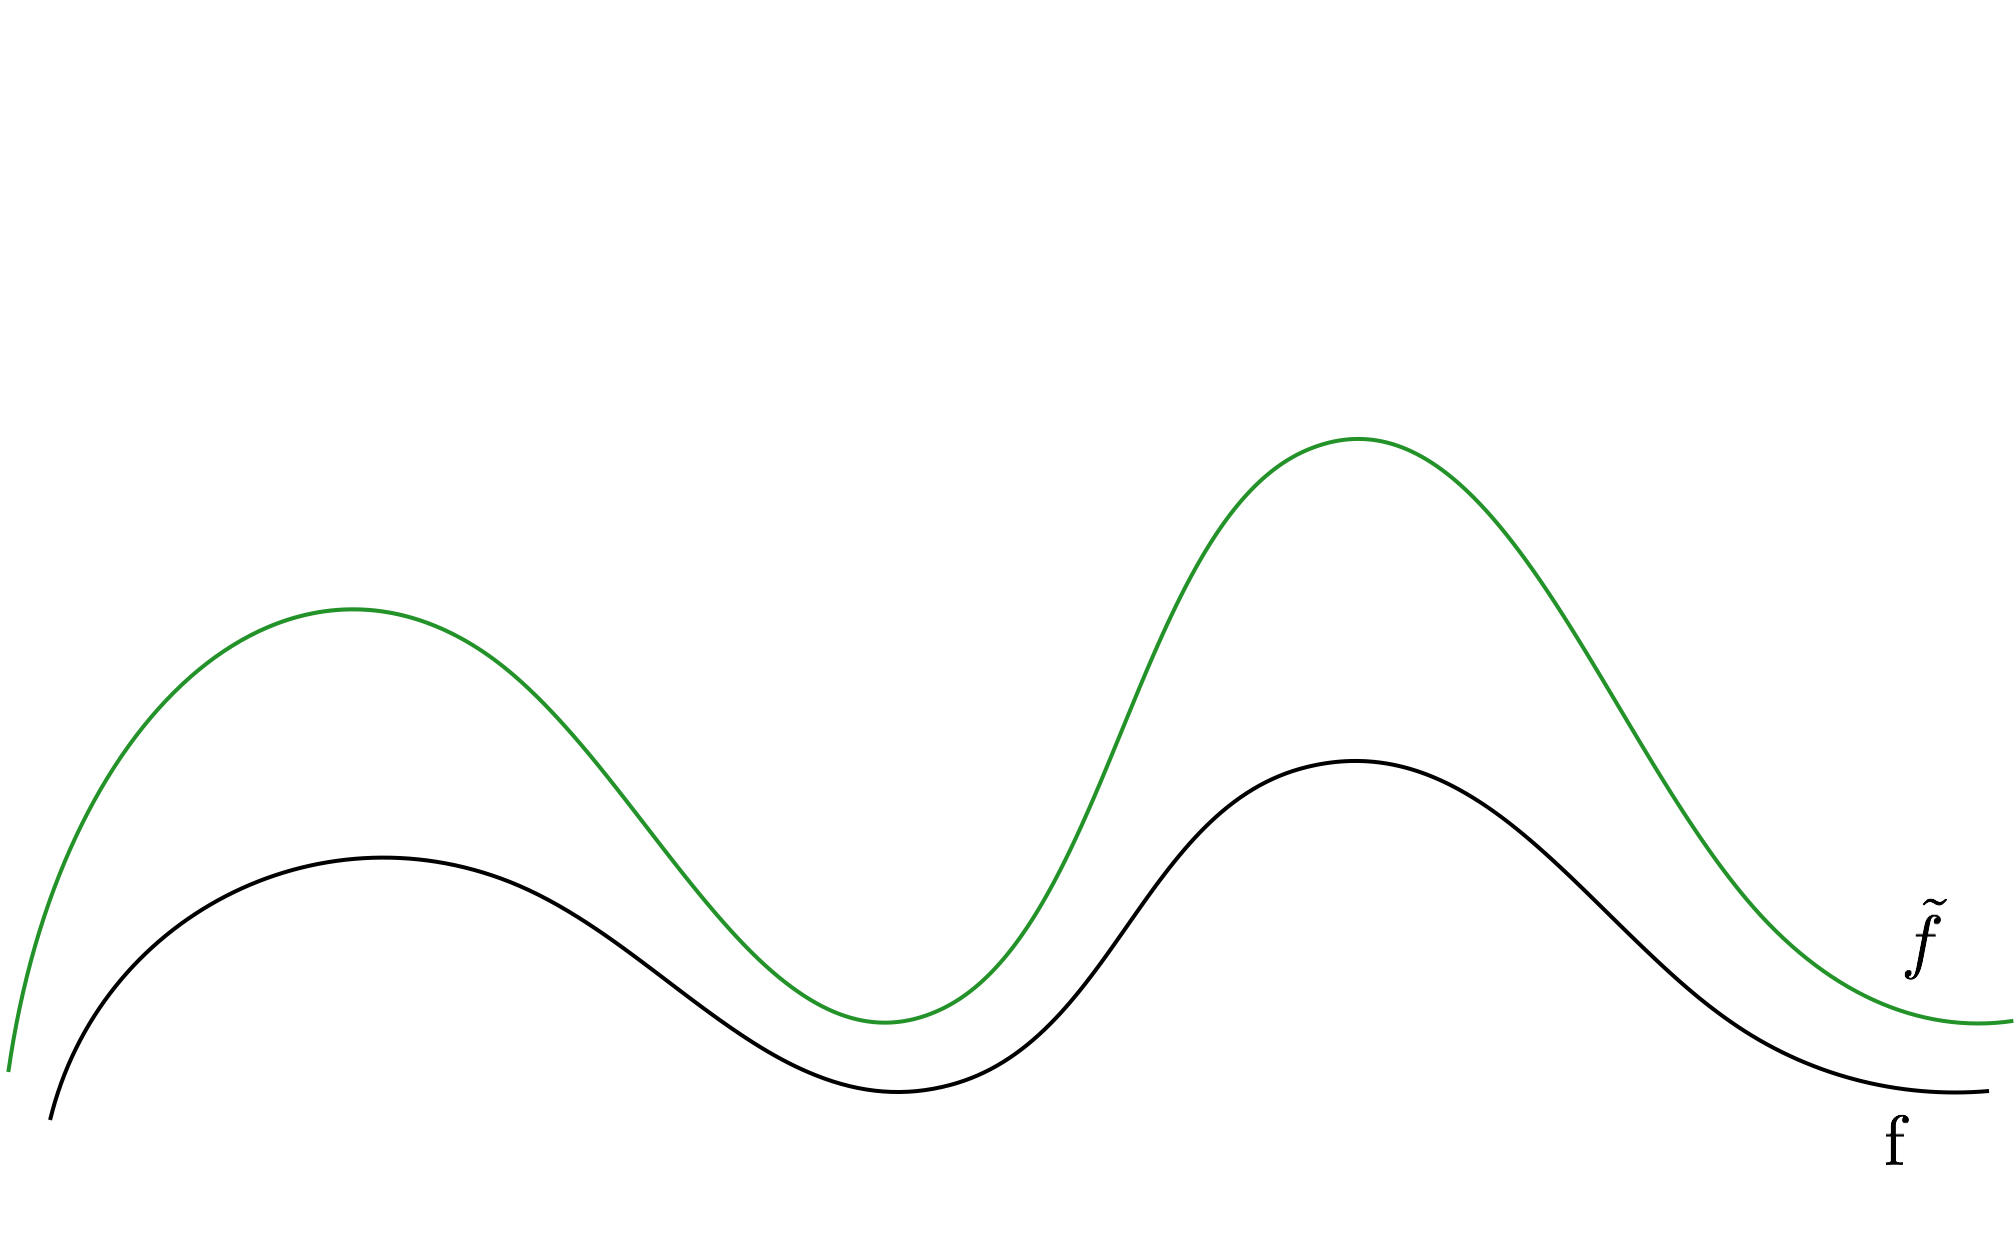
\includegraphics[width=0.8\textwidth]{bothf}
  \end{center}
  \caption{Visualizing just f and $\tilde{f}.$}
\end{figure}



}

\frame{


\begin{figure}
  \begin{center}
    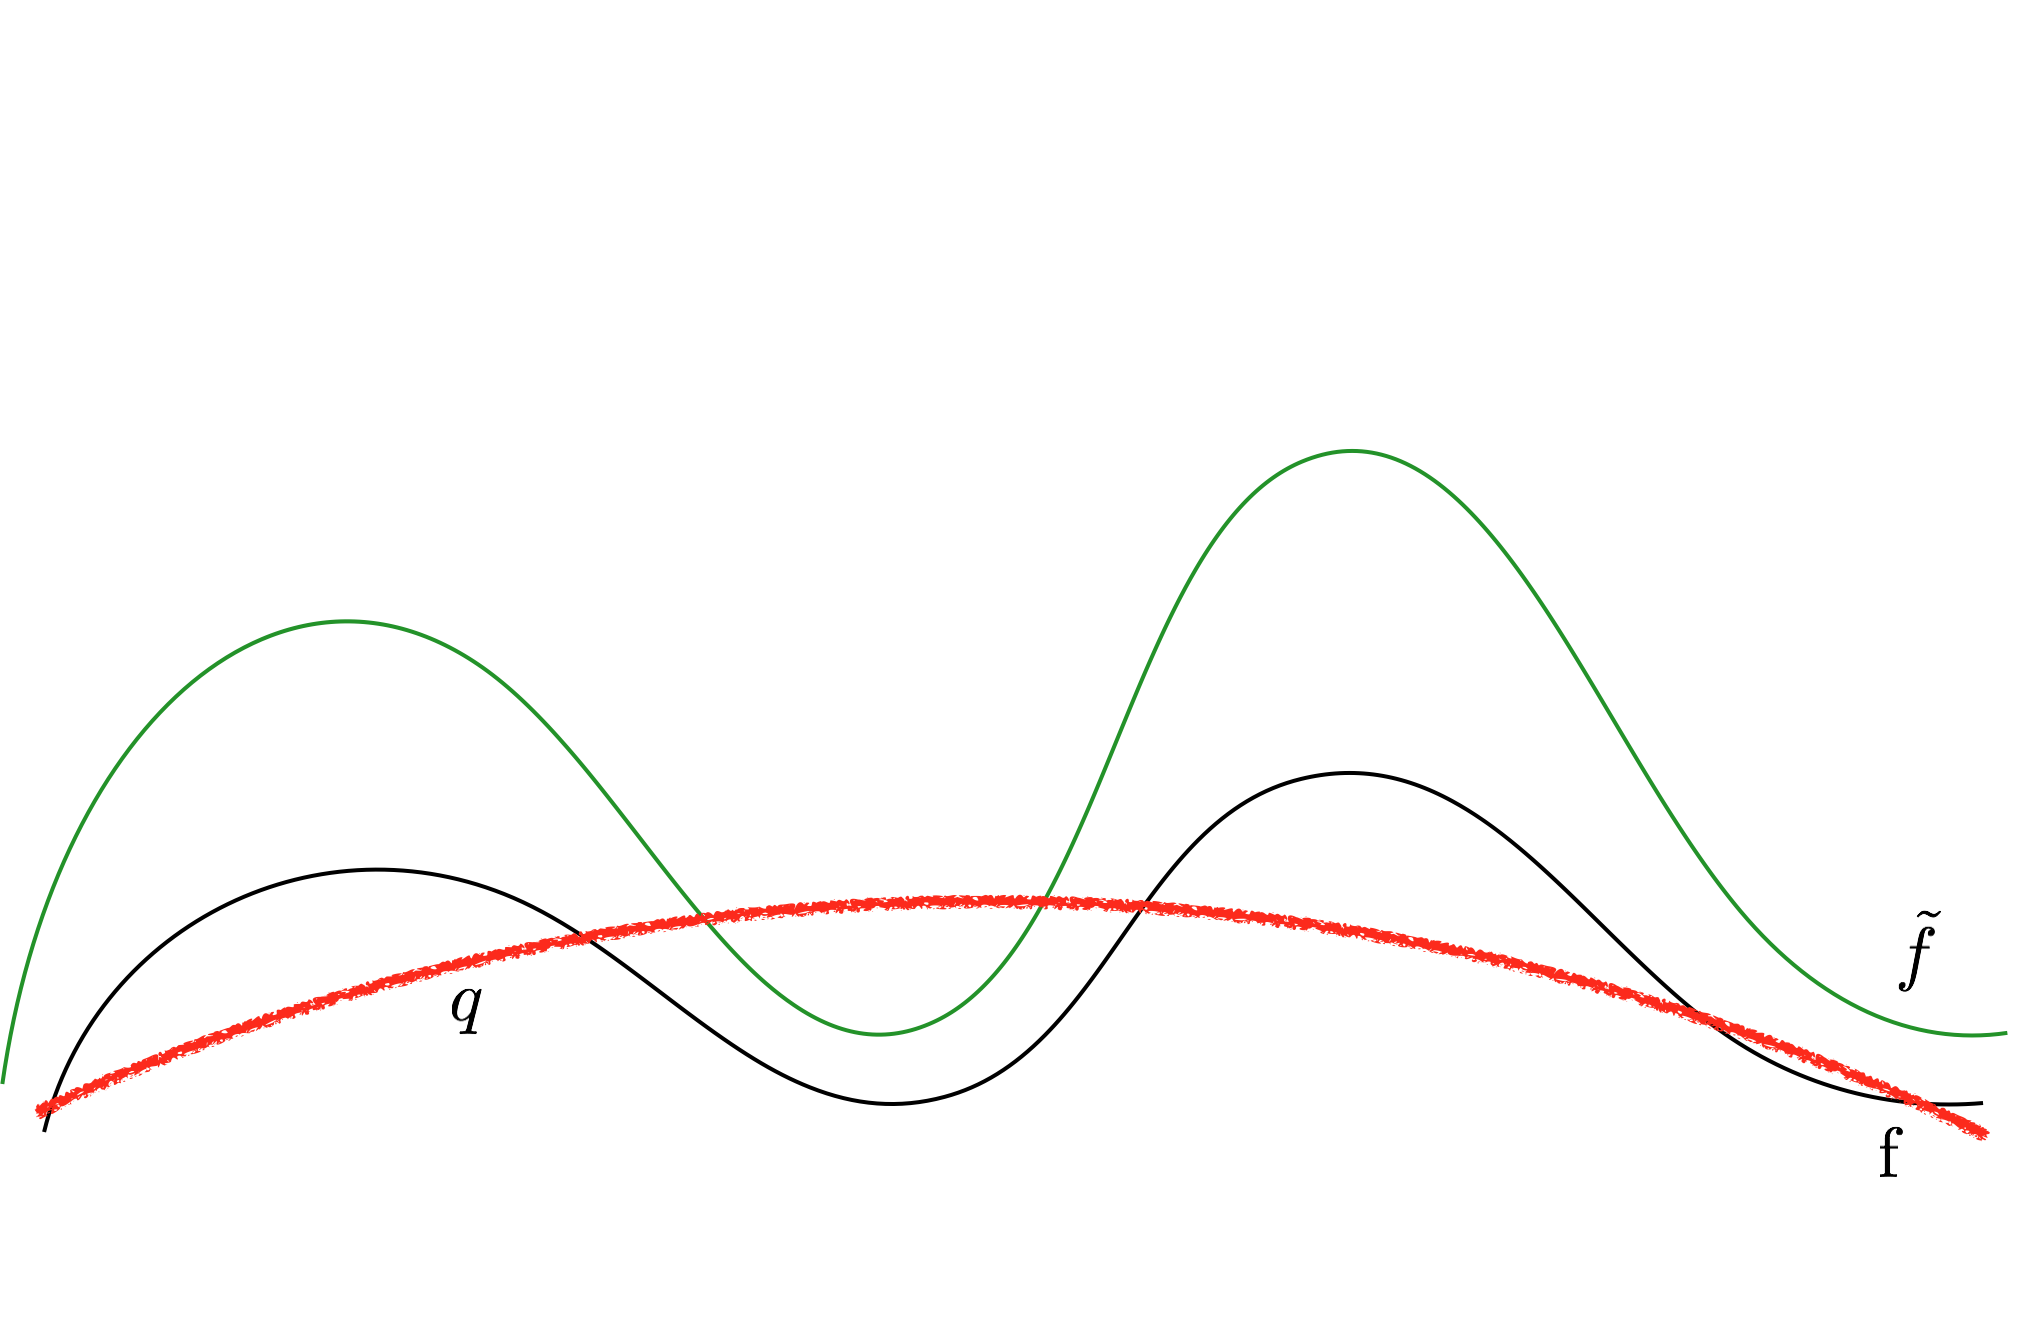
\includegraphics[width=0.8\textwidth]{q}
  \end{center}
  \caption{Visualizing f and $\tilde{f}.$ Now we look at enveloping $q$ over $f.$}
\end{figure}



}

\frame{


\begin{figure}
  \begin{center}
    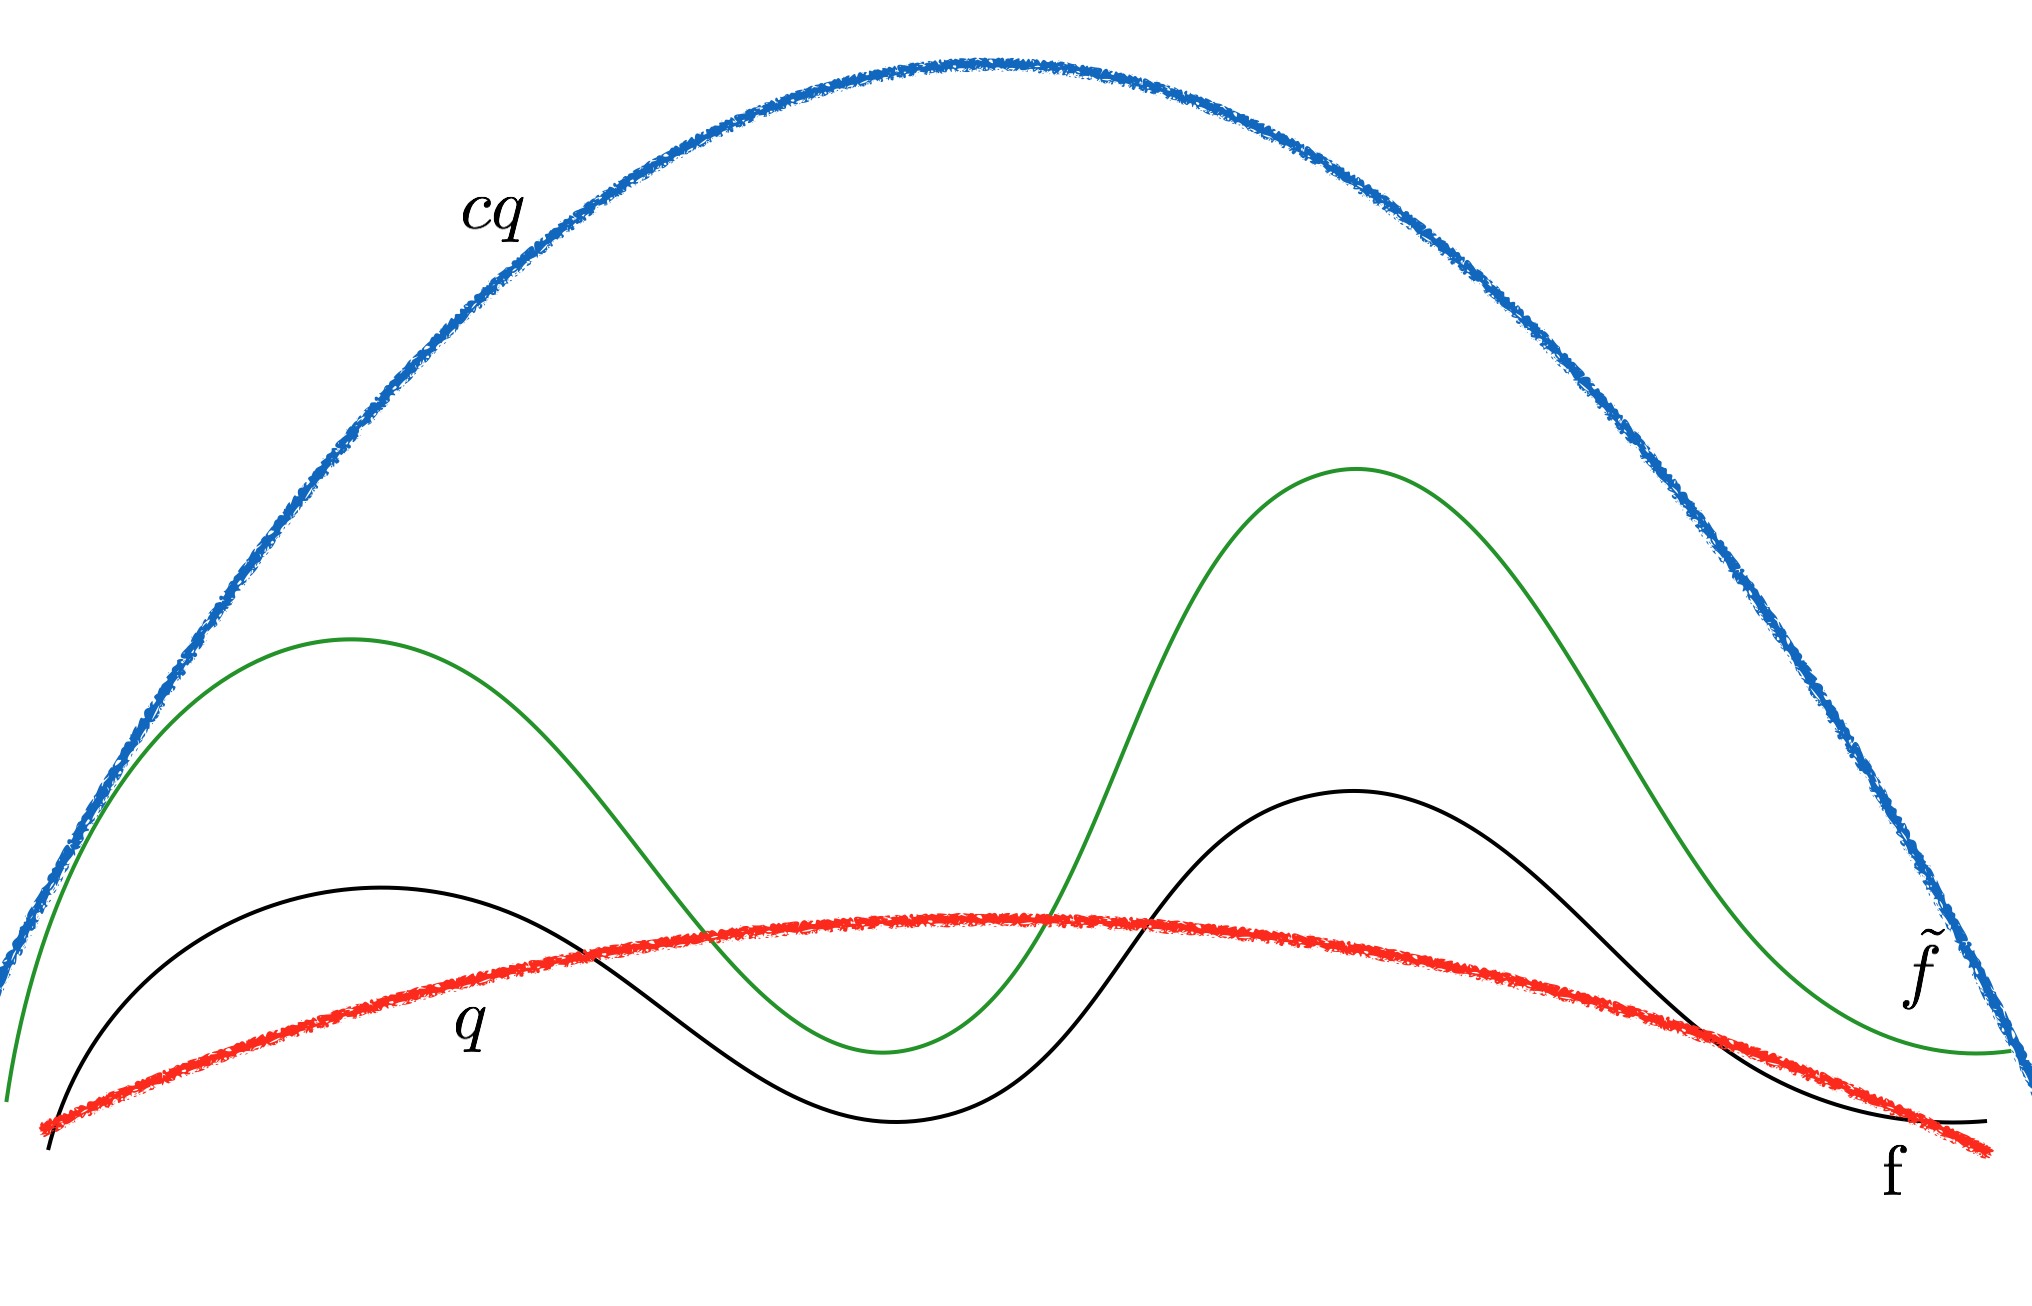
\includegraphics[width=0.8\textwidth]{cq}
  \end{center}
  \caption{Visualizing f and $\tilde{f}.$ Now we look at enveloping $cq$ over $\tilde{f}.$}
\end{figure}



}

\frame{


\begin{figure}
  \begin{center}
    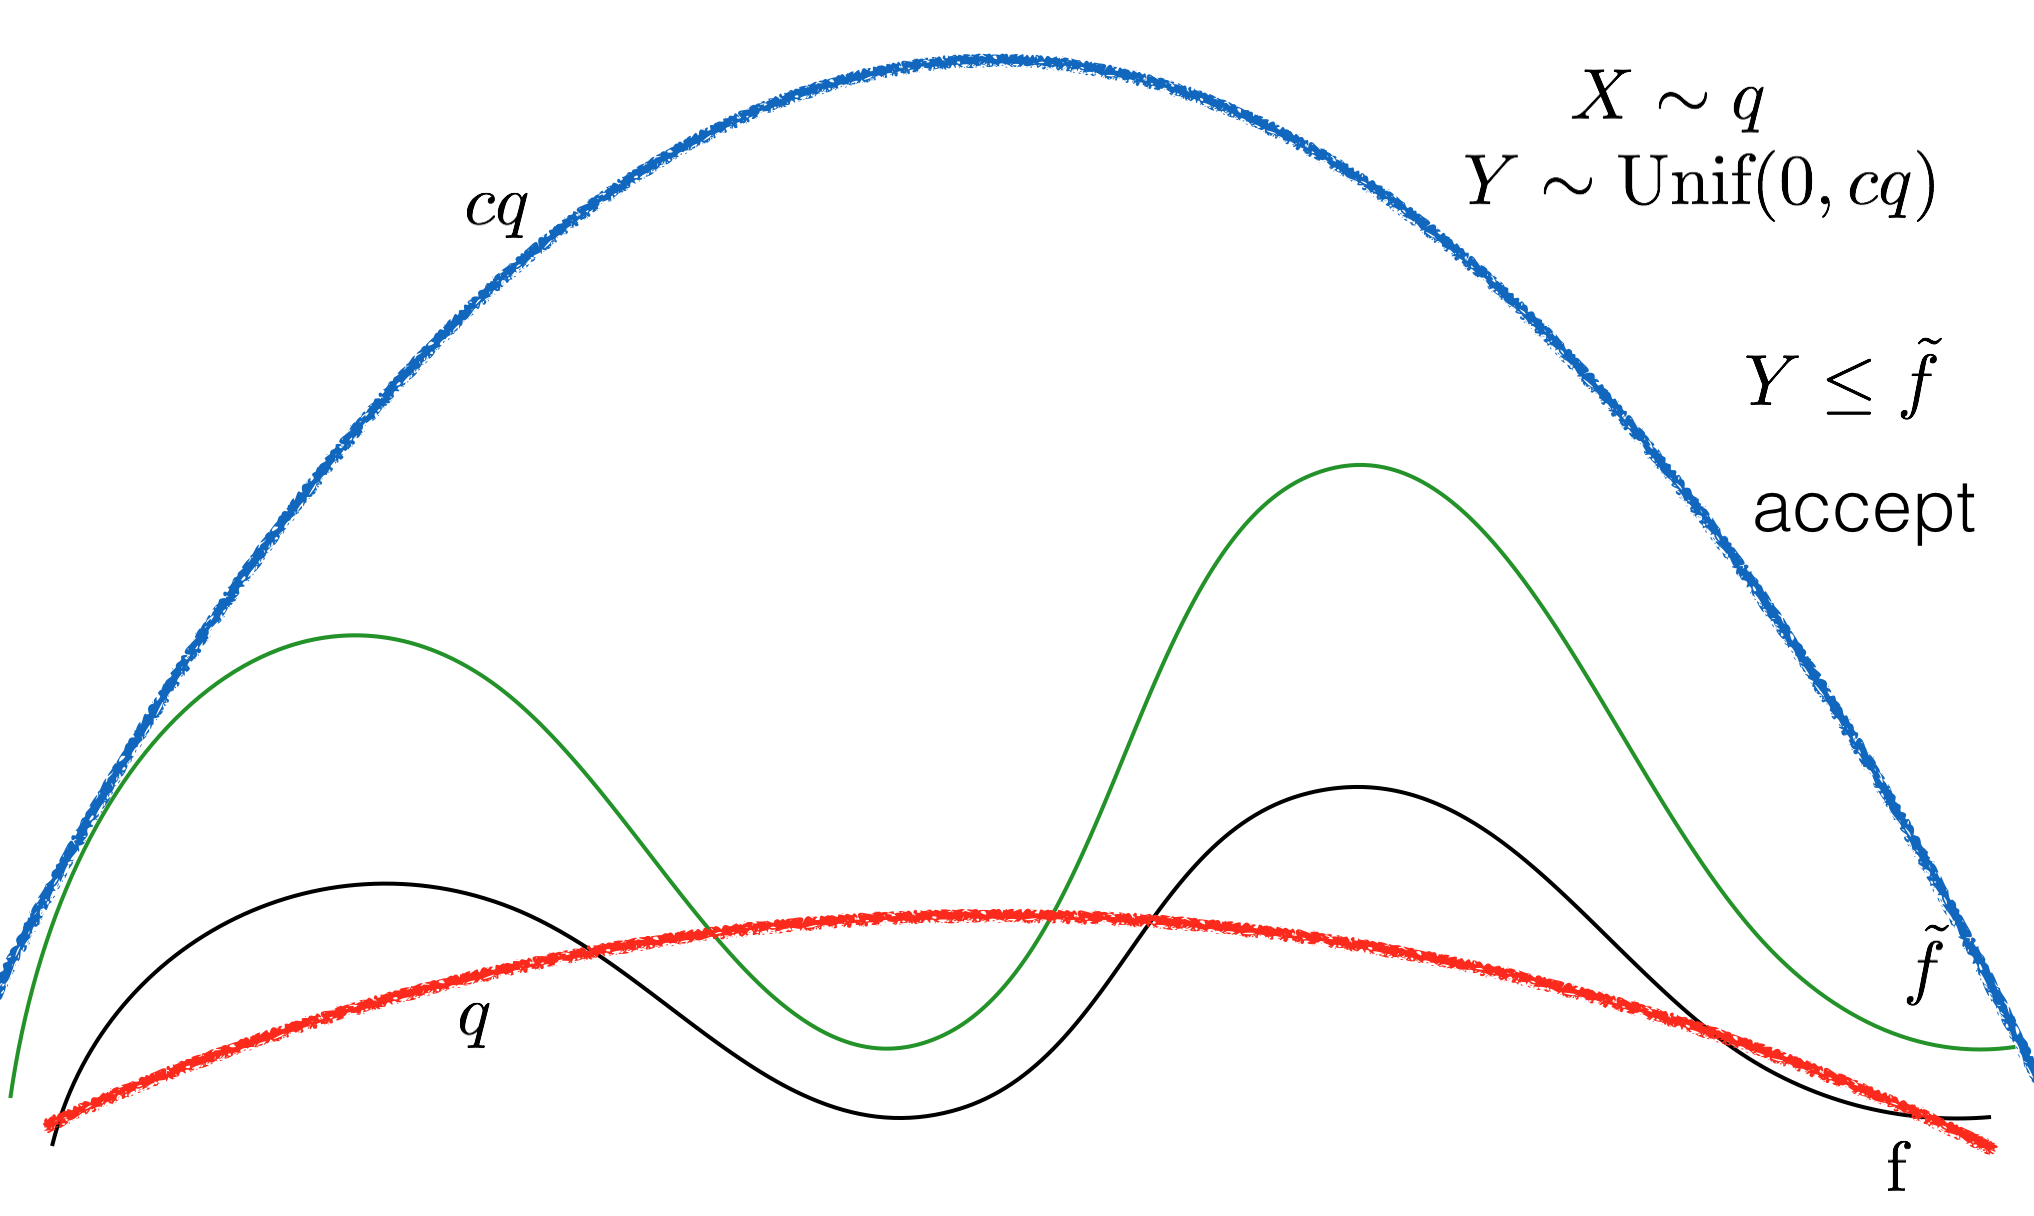
\includegraphics[width=0.8\textwidth]{rejectionAccept}
  \end{center}
  \caption{Recalling the sampling method and accept/reject step.}
\end{figure}



}

\frame{


\begin{figure}
  \begin{center}
    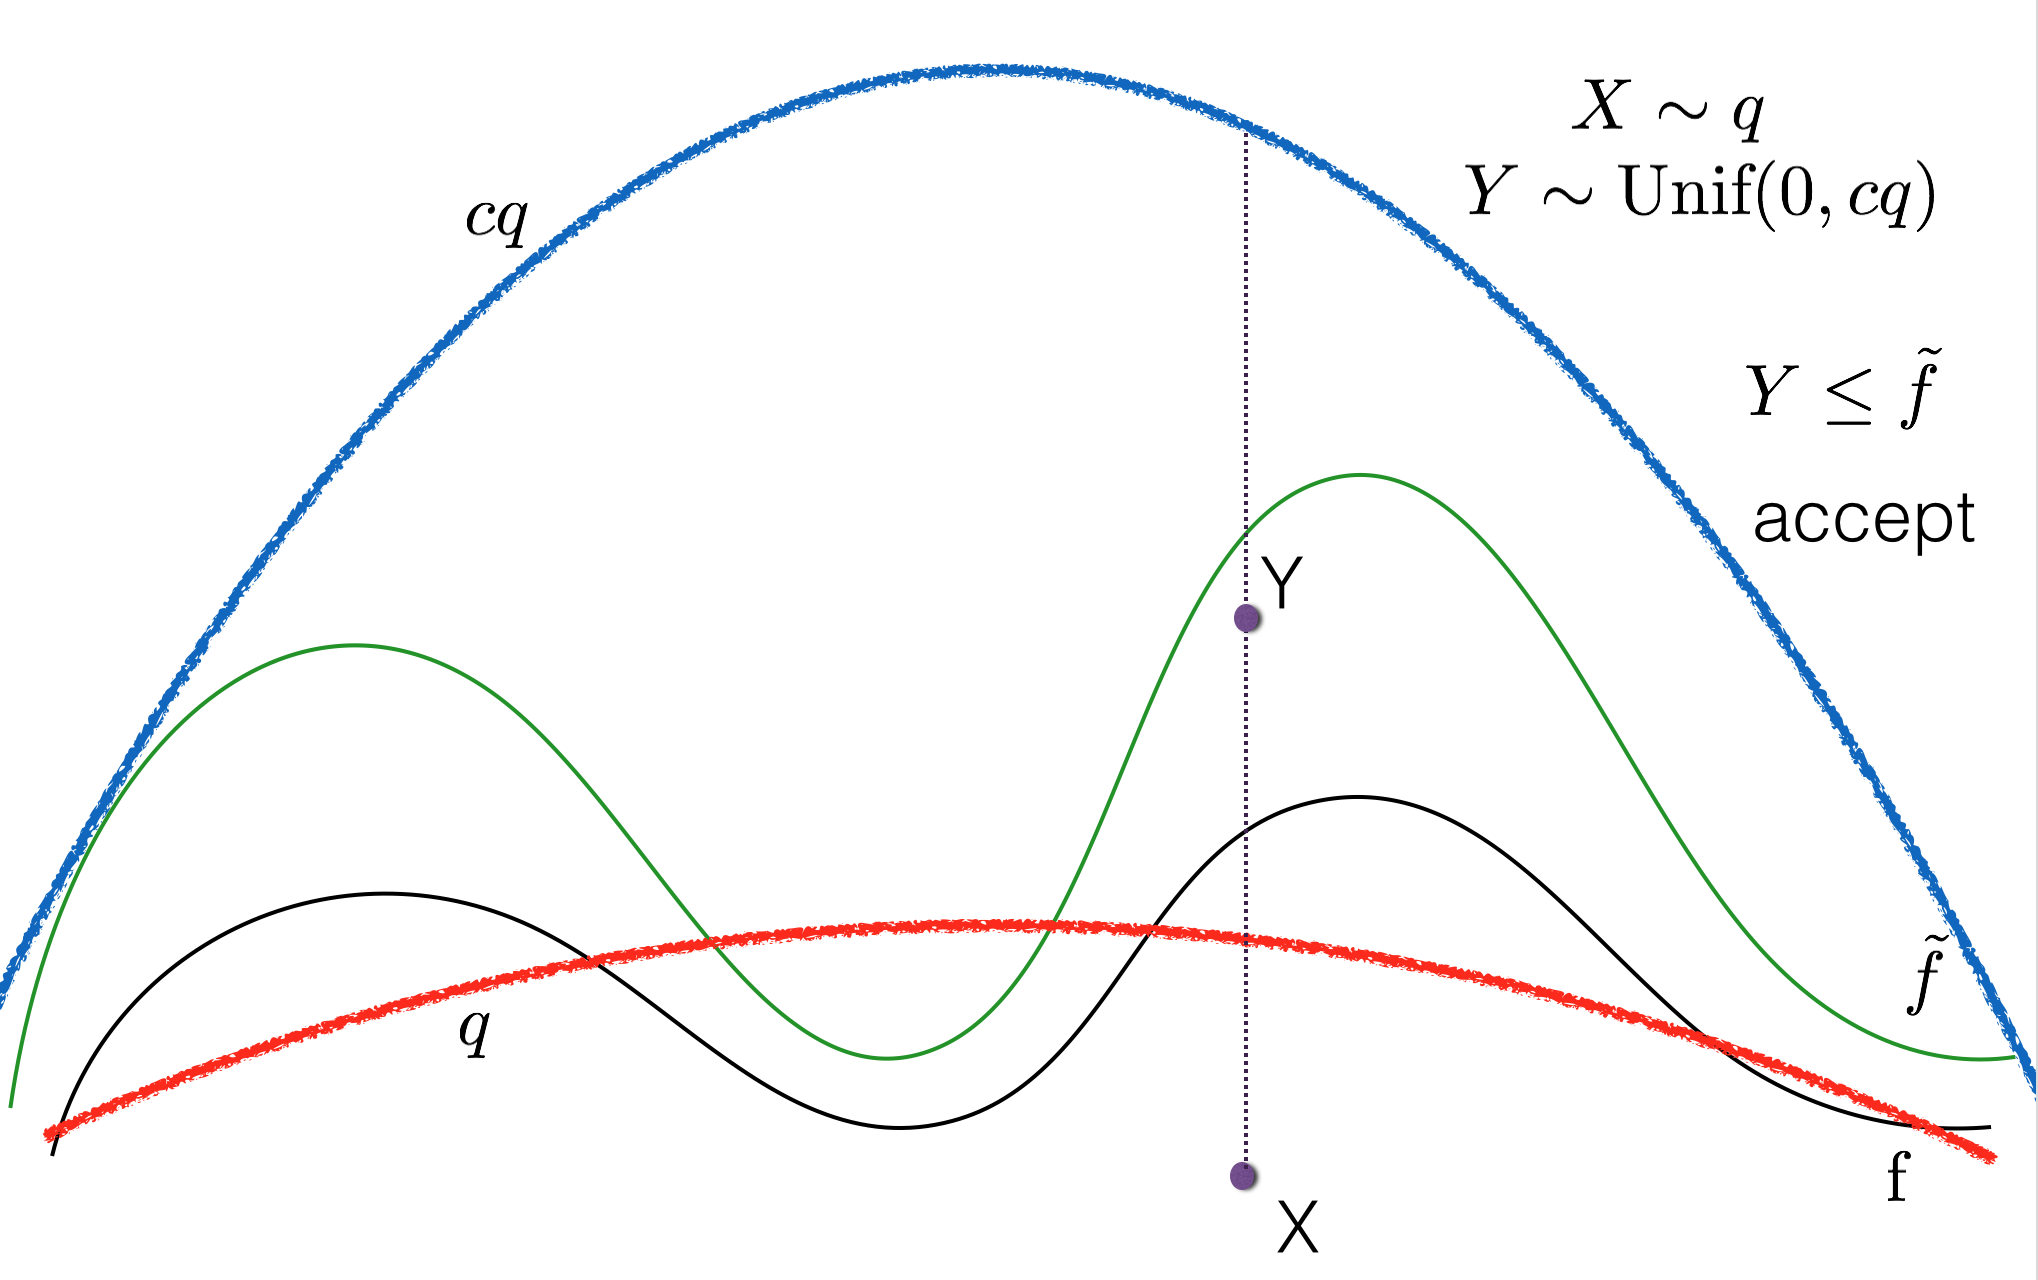
\includegraphics[width=0.8\textwidth]{rejectionAccept2}
  \end{center}
  \caption{Entire picture and an example point $X$ and $Y.$}
\end{figure}



}

\frame{

\begin{itemize}
\item Suppose we want to generate random variables from the Beta(5.5,5.5) distribution. 
\item There are no direct methods for generating from Beta(a,b) if a,b are not integers. 
\item One possibility is to use a Uniform(0,1) as the trial distribution. A better idea is to use an approximating normal distribution. 
\item Do this as an exercise on your own.
\item In lab: you'll go through both importance sampling and rejection sampling.
\end{itemize}
}


%%%start here
%\begin{frame}[fragile]
%\begin{verbatim}
%##simple rejection sampler for Beta(5.5,5.5)
%a <- 5.5; b <- 5.5
%m <- a/(a+b); s <- sqrt((a/(a+b))*(b/(a+b))/(a+b+1))
%funct1 <- function(x) {dnorm(x, mean=m, sd=s)}
%funct2 <- function(x) {dbeta(x, shape1=a, shape2=b)}
%
%##plotting normal and beta densities
%plot(funct1, from=0, to=1, col="blue", ylab="")
%plot(funct2, from=0, to=1, col="red", add=T)
%
%
%##M=1.3 (this is trial and error to get a good M)
%funct1 <- function(x) {1.3*dnorm(x, mean=m, sd=s)}
%funct2 <- function(x) {dbeta(x, shape1=a, shape2=b)}
%plot(funct1, from=0, to=1, col="blue", ylab="")
%plot(funct2, from=0, to=1, col="red", add=T)
%\end{verbatim}
%\end{frame}
%
%%%start here
%\begin{frame}[fragile]
%\begin{verbatim}
%
%##Doing accept-reject
%##substance of code
%set.seed(1); nsim <- 1e5
%x <- rnorm(n=nsim, mean=m, sd=s)
%u <- runif(n=nsim)
%ratio <- dbeta(x, shape1=a, shape2=b) /
%           (1.3*dnorm(x, mean=m, sd=s))
%ind <- I(u < ratio)
%betas <- x[ind==1]
%# as a check to make sure we have enough
%length(betas) # gives 76836
%
%funct2 <- function(x) {dbeta(x, shape1=a, shape2=b)}
%pdf(file = "beta3.pdf", height = 4.5, width = 5)
%plot(density(betas))
%plot(funct2, from=0, to=1, col="red", lty=2, add=T)
%dev.off()
%\end{verbatim}
%\end{frame}
%
%\frame{
%
%\begin{figure}[htbp]
%\begin{minipage}[b]{0.45\linewidth}
%\centering
%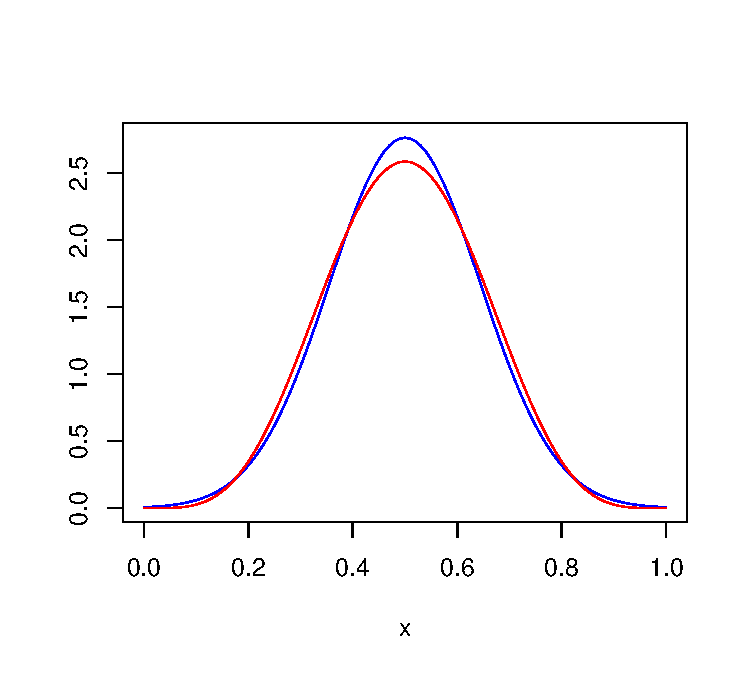
\includegraphics[width=\textwidth]{beta1.pdf}
%\caption{Normal enveloping Beta}
%\label{fig:figure1}
%\end{minipage}
%\hspace{0.5cm}
%\begin{minipage}[b]{0.45\linewidth}
%\centering
%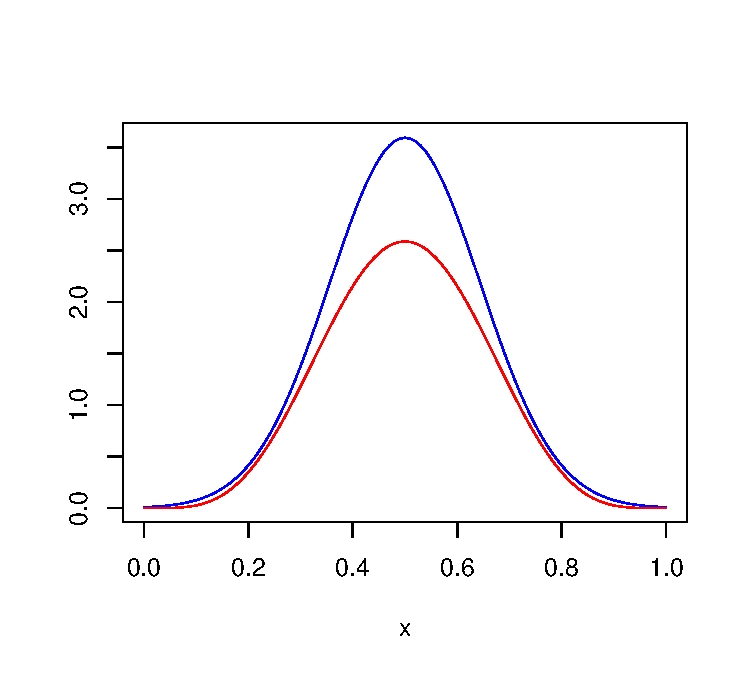
\includegraphics[width=\textwidth]{beta2.pdf}
%\caption{Naive rejection sampling, M=1.3}
%\label{fig:figure2}
%\end{minipage}
%\end{figure}
%
%
%}
%
%
%\frame{
%
%\begin{figure}[htbp]
%\begin{center}
%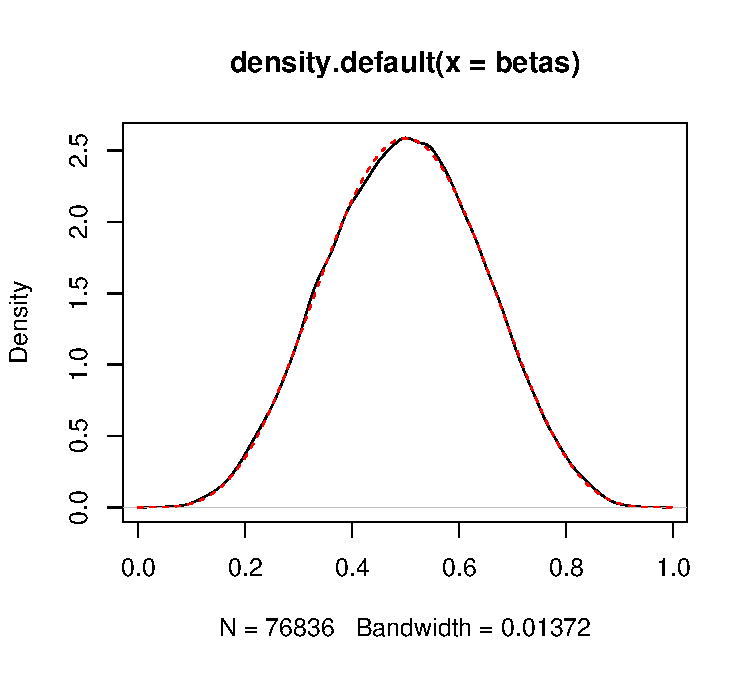
\includegraphics[width=0.5\textwidth]{beta3.pdf}
%\caption{Rejection sampler}
%\label{default}
%\end{center}
%\end{figure}
%
%
%
%}

\end{document}